
%%%%%%%%%%%%%%%%%%%%%%%%%%%%%%%%%%%%%%%%%%%%%%%%%%%%%%%%%%%%%%%%%%%%%%%%%%%%%%%%%%%%%%%
%%%%%%%%%%%%%%%%%%%%%%%%%%%%%%%%%%%%%%%%%%%%%%%%%%%%%%%%%%%%%%%%%%%%%%%%%%%%%%%%%%%%%%%
% 
% This top part of the document is called the 'preamble'.  Modify it with caution!
%
% The real document starts below where it says 'The main document starts here'.

\documentclass[12pt]{article}

\usepackage{amssymb,amsmath,amsthm}
\usepackage[top=1in, bottom=1in, left=1.25in, right=1.25in]{geometry}
\usepackage{fancyhdr}
\usepackage{enumerate}
\usepackage{listings}
\usepackage{graphicx}
\usepackage{float}
\usepackage{multicol}
% Comment the following line to use TeX's default font of Computer Modern.
\usepackage{times,txfonts}
\usepackage{mwe}
\usepackage{caption}
\usepackage{subcaption}
\usepackage{svg}





\makeatletter
\renewcommand*\env@matrix[1][*\c@MaxMatrixCols c]{%
  \hskip -\arraycolsep
  \let\@ifnextchar\new@ifnextchar
  \array{#1}}
\makeatother

\newtheoremstyle{homework}% name of the style to be used
  {18pt}% measure of space to leave above the theorem. E.g.: 3pt
  {12pt}% measure of space to leave below the theorem. E.g.: 3pt
  {}% name of font to use in the body of the theorem
  {}% measure of space to indent
  {\bfseries}% name of head font
  {:}% punctuation between head and body
  {2ex}% space after theorem head; " " = normal interword space
  {}% Manually specify head
\theoremstyle{homework} 

% Set up an Exercise environment and a Solution label.
\newtheorem*{exercisecore}{Exercise \@currentlabel}
\newenvironment{exercise}[1]
{\def\@currentlabel{#1}\exercisecore}
{\endexercisecore}

\newcommand{\localhead}[1]{\par\smallskip\noindent\textbf{#1}\nobreak\\}%
\newcommand\solution{\localhead{Solution:}}

%%%%%%%%%%%%%%%%%%%%%%%%%%%%%%%%%%%%%%%%%%%%%%%%%%%%%%%%%%%%%%%%%%%%%%%%
%
% Stuff for getting the name/document date/title across the header
\makeatletter
\RequirePackage{fancyhdr}
\pagestyle{fancy}
\fancyfoot[C]{\ifnum \value{page} > 1\relax\thepage\fi}
\fancyhead[L]{\ifx\@doclabel\@empty\else\@doclabel\fi}
\fancyhead[C]{\ifx\@docdate\@empty\else\@docdate\fi}
\fancyhead[R]{\ifx\@docauthor\@empty\else\@docauthor\fi}
\headheight 15pt

\def\doclabel#1{\gdef\@doclabel{#1}}
\doclabel{Use {\tt\textbackslash doclabel\{MY LABEL\}}.}
\def\docdate#1{\gdef\@docdate{#1}}
\docdate{Use {\tt\textbackslash docdate\{MY DATE\}}.}
\def\docauthor#1{\gdef\@docauthor{#1}}
\docauthor{Use {\tt\textbackslash docauthor\{MY NAME\}}.}
\makeatother



\usepackage{mathabx}





% Shortcuts for blackboard bold number sets (reals, integers, etc.)
\newcommand{\Reals}{\ensuremath{\mathbb R}}
\newcommand{\Nats}{\ensuremath{\mathbb N}}
\newcommand{\Ints}{\ensuremath{\mathbb Z}}
\newcommand{\Rats}{\ensuremath{\mathbb Q}}
\newcommand{\Cplx}{\ensuremath{\mathbb C}}
%% Some equivalents that some people may prefer.
\let\RR\Reals
\let\NN\Nats
\let\II\Ints
\let\CC\Cplx

%%%%%%%%%%%%%%%%%%%%%%%%%%%%%%%%%%%%%%%%%%%%%%%%%%%%%%%%%%%%%%%%%%%%%%%%%%%%%%%%%%%%%%%
%%%%%%%%%%%%%%%%%%%%%%%%%%%%%%%%%%%%%%%%%%%%%%%%%%%%%%%%%%%%%%%%%%%%%%%%%%%%%%%%%%%%%%%
% 
% The main document start here.

% The following commands set up the material that appears in the header.
\doclabel{Math 614: Homework 10}
\docauthor{Stefano Fochesatto}
\docdate{\today}

\begin{document}


\begin{exercise}{P23} A circulant matrix is one where constant diagonals 'wrap around':

  \begin{figure}[H] 
    \begin{center}  
    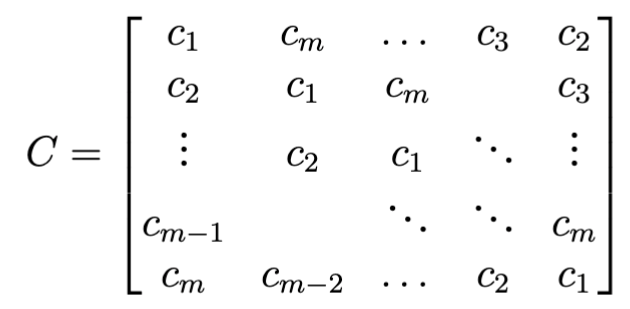
\includegraphics[width = .45\textwidth]{CMatrix.png}  
    \end{center}  
  \end{figure}

  Each entry of $C \in \CC^{mxm}$ is thus a function of hte row/column index difference:
  \begin{equation*}
    C_{jk} =
    \begin{cases} 
      c_{j - k + 1} & j \geq k \\
      c_{m + j - k + 1}& j < k 
   \end{cases}
  \end{equation*}

  Here $c_1, \dots,c_m$ are the entries of a column vector, namely the first column of $C$. Specifying the first column 
  of a circulant matrix describes it completely.\\
  
  Here is an extraordinary fact about circulant matrices: Every circulant matrix has a complete set of eigenvectors that are known in advance, 
  without the eigenvalues. Specifically, define $f_k \in \CC^m$ by, 
  \begin{equation}
    (f_k)_j = exp(-i(j - 1)(k - 1)\dfrac{2\pi}{m})=e^{-i2\pi(k-1)(j-1)/m} \tag{2}
  \end{equation}
  where, as usual $i = \sqrt{-1}$. These vectors are waves, i.e. combinations of familiar sines and cosines.\\
  After some warm-up exercises you will show in part (e) that $cf_k = \lambda_kf_k$.\\
  \begin{enumerate}
    \item[a.] Define the periodic convolution $u * w \in \CC^w$ of vectors $u, w \in \CC^m$ by
    \begin{equation*}
      (u*w)_j = \sum_{k = 1}^m u_{\mu(j,k)}w_k
    \end{equation*}  
    where, 
    \begin{equation*}
      \mu_{(j,k)} = 
      \begin{cases}
        j - k + 1 & j \geq k\\
        m + j - k + 1 & j < k 
      \end{cases}
    \end{equation*}
    Show that $u*w = w*u$.\\

    \solution Suppose the following periodic convolution for some row $j$, and let the $|$ denote where we 'wrap-around' indices with respect to the function $\mu$,
    \begin{equation*}
      (u*w)_j = \sum_{k = 1}^m u_{\mu(j,k)}w_k = u_jw_1 + u_{j-1}w_2 + u_{j-3}w_3 \dots u_1w_j| + u_mw_{j+1} + u_{m-1}w_{j+2} \dots u_{j+1}w_{m}.
    \end{equation*}
    Now consider $(w*u)_j$,
    \begin{equation*}
      (w*u)_j = \sum_{k = 1}^m w_{\mu(j,k)}u_k = w_ju_1 + w_{j-1}u_2 + w_{j-3}u_3 \dots w_1u_j| + w_mu_{j+1} + w_{m-1}u_{j+2} \dots w_{j+1}u_{m} .
    \end{equation*}
    Note that if we reverse the indices of the partial sum before and after the $|$ we get the same sum as $(u*w)_j$. Said another way we can reverse the indices of each partial sum to get 
    the following, 
    \begin{equation*}
      \sum_{k = 1}^j u_{j - k + 1}w_k = \sum_{k = 1}^j w_{j - k + 1}u_k,
    \end{equation*}
    \begin{equation*}
      \sum_{k = j+1}^m u_{m + j - k + 1}w_k = \sum_{k = j+1}^m w_{m + j - k + 1}u_k.
    \end{equation*}
    Finally by splitting up the periodic convolution and applying substitution we get the following, 
    \begin{align*}
      (u*w)_j &= \sum_{k = 1}^m u_{\mu(j,k)}w_k \\
      &= \sum_{k = 1}^j u_{j - k + 1}w_k + \sum_{k = j+1}^m u_{m + j - k + 1}w_k,\\
      &= \sum_{k = 1}^j w_{j - k + 1}u_k + \sum_{k = j+1}^m w_{m + j - k + 1}u_k,\\
      &= \sum_{k = 1}^m w_{\mu(j,k)}u_k, \\
      &=  (w*u)_j.
    \end{align*}

    \vspace{1in}



%% REview this one later
    \item[b.] Show that $Cu = v*u$ if $C$ is a circulant matrix and $v$ is the first column of $C$.
    \solution Suppose that $C \in \CC^{mxm}$ is a circulant matrix where $v$ is the first column and let 
    $u$ be some vector in $\CC^{m}$ . Consider the convolution $v*u$ and by part a, it's $j$th entry is given by, 
    \begin{equation*}
      (v*u)_j = \sum_{k = 1}^m v_{\mu(j,k)}u_k = v_ju_1 + v_{j-1}u_2 + v_{j-3}u_3 \dots v_1u_j| + v_mu_{j+1} + v_{m-1}u_{j+2} \dots v_{j+1}u_{m}.
    \end{equation*}
    Now consider the $j$th entry in the $Cu$ matrix-vector product, and note that since $C$ is a circular matrix the $j$th row is defined by the 
    row/column index difference defined in the first part of this problem, so
    \begin{equation*}
      (Cu)_j = \sum_{k = 1}^m C_{jk}u_k = \sum_{k = 1}^m v_{\mu(j,k)}u_k = (v*u)_j. 
    \end{equation*}
    \vspace{1in}




    \item[c.] Show that the vectors defined in (2) are orthogonal. \\
    \solution Consider two arbitrary eigenvectors $f_u,f_v$ defined by (2). By (2) we can defined the innerproduct between them to be, 
    \begin{equation*}
      f_u^*f_v = \sum_{j = 1}^m (f_u)_j(f_v)_j.
    \end{equation*}
    Applying our definition of the eigenvector entries in (2) and simplifying we get the following, 
    \begin{align*}
      f_u^*f_v &=\sum_{j = 1}^m (f_u)_j(f_v)_j,\\
      &=\sum_{j = 1}^m e^{\frac{-i 2 \pi (u - 1)(j - 1)}{m}}e^{\frac{-i 2 \pi (v - 1)(j - 1)}{m}},\\
      &=\sum_{j = 1}^m e^{\frac{(-i 2 \pi (u - 1) (j - 1)) +(-i 2 \pi (v - 1) (j - 1))}{m}},\\
      &=\sum_{j = 1}^m e^{-i 2 \pi (j-1) \frac{(u - 1) + (v - 1)}{m} },\\
      &=\sum_{j = 1}^m e^{-i 2 \pi \frac{(u + v - 2)}{m}^{(j-1)}},\\
      &=\sum_{j = 0}^{m-1} e^{-i 2 \pi \frac{(u + v - 2)}{m}^{j}}.
    \end{align*}
    Note that we have a finite geometric sum, writing it in a closed form results in, 
    \begin{align*}
      f_u^*f_v &= \dfrac{1 - e^{-i 2 \pi \frac{(u + v - 2)}{m}^{m}}}{1 - e^{-i 2 \pi \frac{(u + v - 2)}{m}}},\\
       &= \dfrac{1 - e^{-i 2 \pi (u + v - 2)}}{1 - e^{-i 2 \pi \frac{(u + v - 2)}{m}}}.
    \end{align*}
    Writing the numerator in-terms of sin and cos we get the following, 
    \begin{equation*}
      f_u^*f_v = \dfrac{1 - \cos(2\pi(u+v - 2)) + i\sin(2\pi(u+v - 2))}{1 - e^{-i 2 \pi \frac{(u + v - 2)}{m}}}.
    \end{equation*}
    Note that the sin term will always go to zero, since it will always have as an input a multiple of $2\pi$. Similarly the cos
    term will return a 1. Therefore the numerator goes to 0 and we get the $f_u$ and $f_v$ are orthogonal. 

    \vspace{1in}


    \item[d.] For $m = 20$, use Matlab to plot the real parts of the vectors $f_1, \dots f_5$ together in a single figure.\\
    \solution It seems as though I was unable to generate the right eigenvalues with the following script which implements the given formula, \\
     \textbf{Code:}
     \begin{center}
     \lstinputlisting{P23d.txt}
     \end{center} 
     \textbf{Console:}
     \begin{center}
     \lstinputlisting[basicstyle = \footnotesize ]{P23dVectors.txt}
     \end{center} 
     Clearly the real parts of these eigenvectors will plot a straight line, nothing resembling a discretizing wave. I'm not really sure what is wrong with my code so I'll continue 
     by generating a circulant matrix 
     then calling eig() on it to get usable vectors,\\
     \textbf{Console:}
     \begin{center}
     \lstinputlisting{P23dRand.txt}
     \end{center}   
      \begin{figure}[H] 
        \begin{center}  
        \caption{Real Parts of Circulant Matrix Eigenvectors}  
        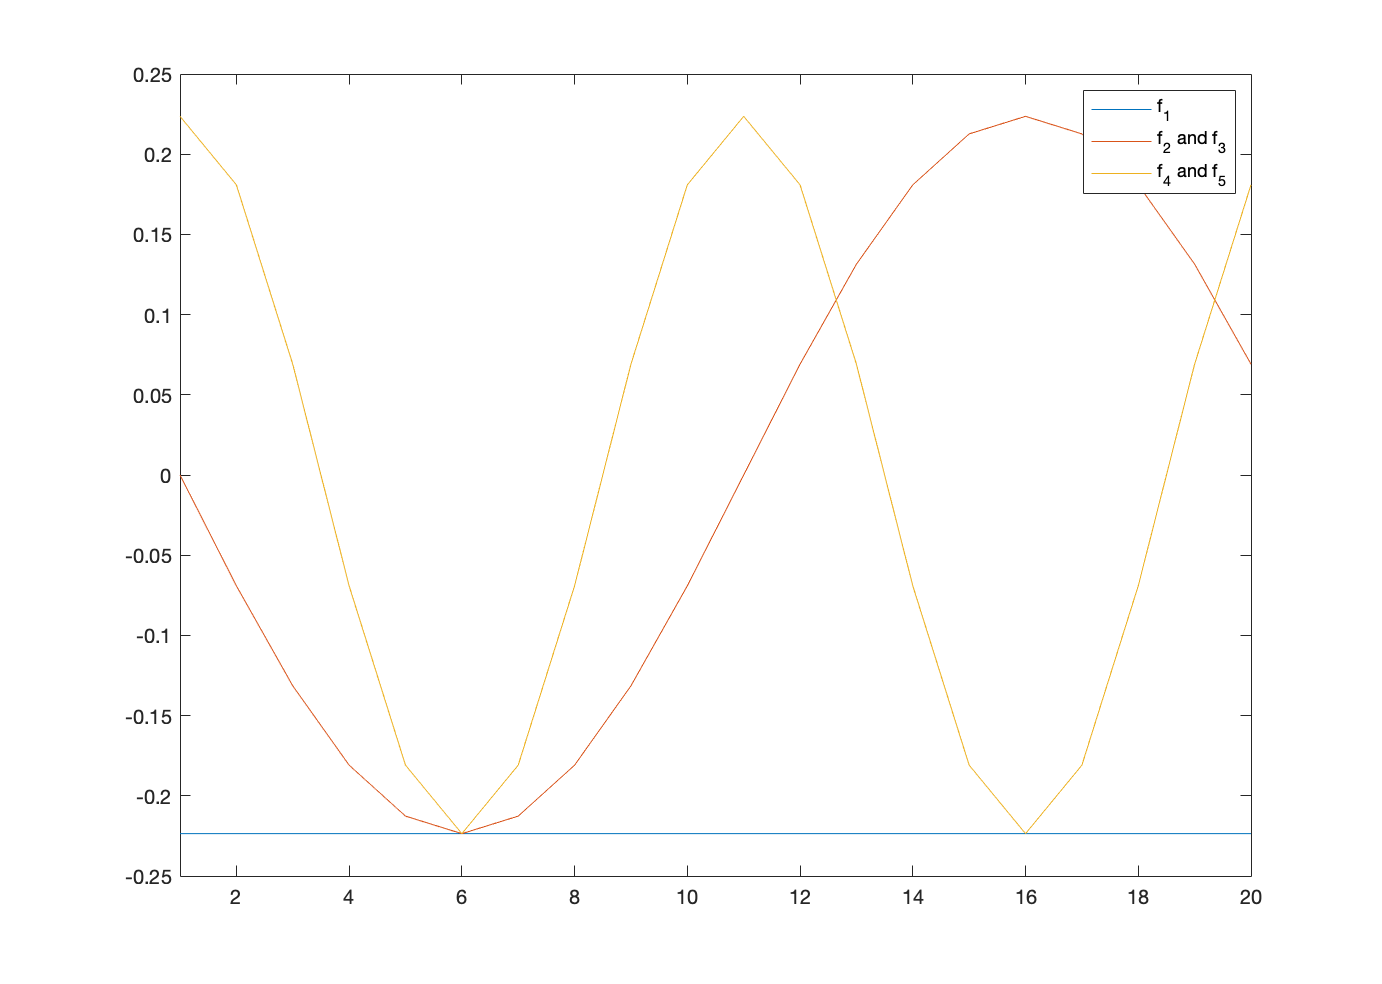
\includegraphics[width = \textwidth]{P23d.png}  
        \end{center}  
      \end{figure}
    \vspace{1in}
      


    \item[e.] For the general circulant matrix $C$ in (1) above, give a formula for the eigenvalues $\Lambda_k$, in terms of the entries $c_1,\dots c_m$.
    that is, show via by-hand calculation that, 
    \begin{equation*}
      Cf_k = \lambda_kf_k.
    \end{equation*}  

    \solution Recall from part $b$ that the matrix-vector product $Cfi$ can be rewritten as the convolution $c*fi$ where $c$ is the first column of $C$.
    Doing so we get the following, 
    \begin{equation*}
      (Cfi)_j = (c*fi)_j = (fi*c)_j = \sum_{k = 1}^j fi_{j - k + 1}c_k + \sum_{k = j+1}^m fi_{m + j - k + 1}c_k.
    \end{equation*} 
    Recall the definition of the $fk_j$ term from (2), we can factor an $fi_j$ term from each sum we get the following,
    \begin{equation*}
      (Cfi)_j = fi_j \left(\sum_{k = 1}^j \dfrac{fi_{j - k + 1}}{fi_j}c_k + \sum_{k = j+1}^m \dfrac{fi_{m + j - k + 1}}{fi_j}c_k\right).
    \end{equation*}
    Applying our definition of each term of the eigenvector from (2) we get, 
    \begin{align*}
      (Cfi)_j &= fi_j \left(\sum_{k = 1}^j \dfrac{fi_{j - k + 1}}{fi_j}c_k + \sum_{k = j+1}^m \dfrac{fi_{m + j - k + 1}}{fi_j}c_k\right).\\
      &= fi_j \left(\sum_{k = 1}^j \dfrac{e^{-i 2 \pi (i - 1) (j - k + 1 - 1)(1/m)}}{e^{-i 2 \pi(i - 1)(j - 1) (1/m) }}c_k + \sum_{k = j+1}^m \dfrac{e^{-i 2 \pi (i - 1) (m + j - k + 1 - 1)(1/m)}}{e^{-i 2 \pi(i - 1)(j - 1)(1/m)}}c_k\right).\\
      &= fi_j \left(\sum_{k = 1}^j e^{-i 2 \pi (1/m) (i - 1) (j - k - j + 1)} c_k + \sum_{k = j+1}^m e^{-i 2 \pi (1/m) (i - 1) (m + j - k - j + 1)} c_k \right),\\
      &= fi_j \left(\sum_{k = 1}^j e^{-i 2 \pi (1/m) (i - 1) (1 - k) } c_k + \sum_{k = j+1}^m e^{-i 2 \pi (1/m) (i - 1) (m - k + 1)} c_k \right),
    \end{align*}
    \dots I got very stuck here. This felt right but I couldn't get the sum back together.
    \vspace{1in}

    \item[f.] Download the circu.m matlab script, and generate a circulant matrix $C$ with the first column consisting of 20 random numbers of your choice. 
    Use the result of $(e)$ to compute the eigenvalues $\lambda_k$, and compare these against the result of eig(). Also generate $f_5$ from (2) and verify that 
    $cf_5 = \Lambda_5f_5$ to high accuracy; use a vector norm. \\
    \solution  I'm not sure what was going on with part d and e. I was able to play around with the circu.m script and some formulas I found online for how the eigenvalues and eigenvectors should be 
    calculated. 



     
  \end{enumerate}
  
\end{exercise}
\vspace{1in}



\begin{exercise}{22.1} Show that for Gaussian elimination with partial pivoting applied to any matrix $A \in \CC^{mxm}$, the growth factor (22.2) satisfies
  $\rho \leq 2^{m-1}$.\\
  \solution Suppose a matrix $A \in \CC^{mxm}$, and recall that partial pivoting will not change $\max_{i,j}|a_{i,j}|$. Applying the first step (or L factor) in gaussian elimination to 
  the matrix $A$ we get a reduced matrix $A_1$ with zeroes below the diagonal of the first column whose entries can be described by the following, 
  \begin{equation*}
    a^1_{i,j} = a_{i,j} - \dfrac{a_{i, 1}}{a_{1,1}}a_{i,1}.
  \end{equation*}
  Recall that partial pivoting ensures us that, 
  \begin{equation*}
    \dfrac{a_{i, 1}}{a_{1,1}} \leq 1.
  \end{equation*}
  Thus by substitution we obtain the following inequality, 
  \begin{equation*}
    |a^1_{i,j}| = |a_{i,j} - \dfrac{a_{i, 1}}{a_{1,1}}a_{i,1}| \leq |a_{i,j} + \dfrac{a_{i, 1}}{a_{1,1}}a_{i,1}|  \leq |a_{i,j} + a_{i,1}| \leq 2 \max_{i,j}|a_{i,j}|.
  \end{equation*}
  We will continue via induction on the $k$th iteration of gaussian elimination with partial pivoting. Let $a^k_{i,j}$ denote the entries of the reduced matrix $A_k$ obtained through $k$ iterations of gaussian elimination. Following the last inequality we get, 
  \begin{equation*}
    a^{k+1}_{i,j} = a^{k}_{i,j} - \dfrac{a^{k}_{i, k+1}}{a^{k}_{k+1,k+1}}a^{k}_{i,k+1}.
  \end{equation*}
  Again since the matrix has already been pivoted we know the following, 
  \begin{equation*}
    \dfrac{a^{k}_{i, k+1}}{a^{k}_{k+1,k+1}} \leq 1.
  \end{equation*}
  Therefore, similarly to the base case, by substitution it follows that, 
  \begin{equation*}
    |a^{k+1}_{i,j}| \leq |a^{k}_{i,j} + a^{k}_{i,k+1}| \leq 2 \max_{i,j}|a^k_{i,j}|.
  \end{equation*}
  Since there are $m-1$ iterations to perform gaussian elimination on an $mxm$ matrix we get that  $|a^{m-1}_{i,j}| = |u_{i,j}|$. From our induction argument we can chain the inequalities to get, 
  \begin{equation*}
    |u_{i,j}| \leq 2 \max_{i,j}|a^{m-2}_{i,j}| \leq 2^2 \max_{i,j}|a^{m-3}_{i,j}| \leq \dots \leq 2^{m-1}|a_{i,j}|.
  \end{equation*}
  Which gives us that, 
  \begin{equation*}
    \dfrac{|u_{i,j}|}{|a_{i,j}|} \leq 2^{m-1}.
  \end{equation*}
\end{exercise}
\vspace{1in}


\begin{exercise}{22.2} Experiment with solving 60 x 60 systems of equation $Ax = b$ by Gaussian elimination with partial pivoting, with 
  $A$ having the form in 22.4. Do you observe that the results are useless because of the growth factor of order $2^60$? At your first attempt you 
  may not observe this, because the integer entries of $A$ may prevent any rounding errors from occurring. If so, find a way to modify your problem slightly so that 
  the growth factor is the same or nearly so and catastrophic rounding error really do take place. \\
  \solution The following matlab script constructs a 60x60 matrix with the form found in 22.4. We then performed gaussian elimination on 20 random vectors, each with a maximum 
  range double the previous one. This was done in order to observe a wider range of $x$ solutions since the text mentions that a growth factor on the order of $2^{60}$ corresponds to 
  a loss of about 60 bits of precision. We then computed the solution using the $\backslash$ operator, although any of our previous methods for solving systems should do fine as well.\\
  \textbf{Code:}
  \begin{center}
  \lstinputlisting{22p2.txt}
  \end{center} 
  \begin{figure}[H] 
    \begin{center}  
    \caption{Maximum Input Size vs Error}  
    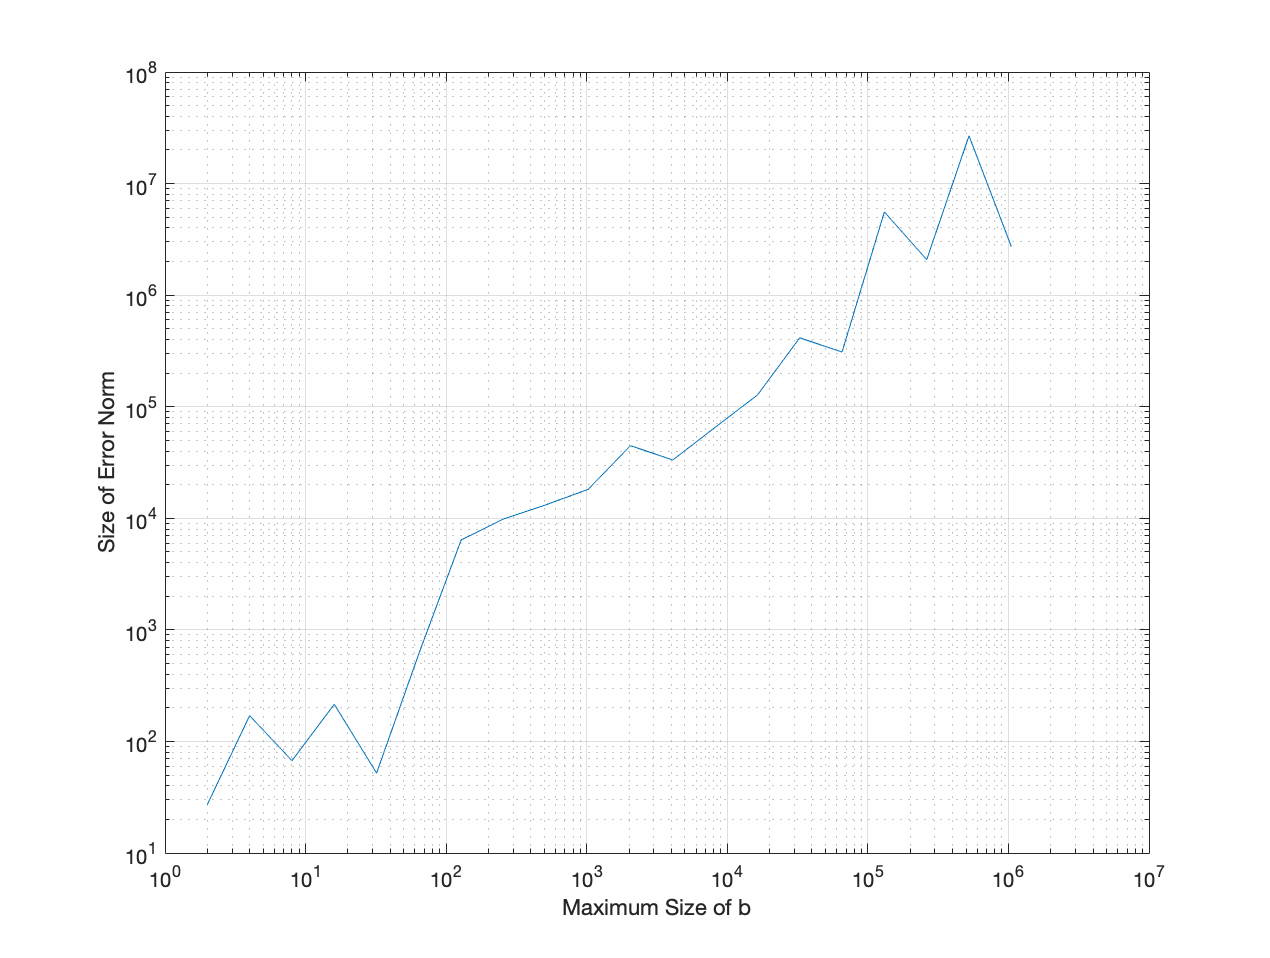
\includegraphics[width = \textwidth]{ErrorAnalysis.png}  
    \end{center}  
  \end{figure}
  As we can see, when given digits to loose this method of solving this specific system will loose them. 
  
\end{exercise}



\vspace{1in}



\begin{exercise}{23.2} Use the proof of Theorem 16.2 as a guide, derive Theorem 23.3 from Theorems 23.2 and 17.2.\\
  \solution Let $A \in \CC^{mxm}$ be hermitian positive definite, and let a Cholesky factorization of $A$ be computed by algorithm 23.1
  on a machine satisfying 13.1 and 13.7. By Theorem 23.2 this Cholesky factorization exists such that the computed $\tilde{R}$ satisfies, 
  \begin{equation*}
    \tilde{R}^*\tilde{R} = A + \delta A, 
  \end{equation*}
  where, 
  \begin{equation*}
    \dfrac{||\delta A||}{||A||} = O(\epsilon_{machine}).
  \end{equation*}
  Recall that Theorem 17.2 states that solving systems via backwards substitution (and forwards substitution) is backwards stable such that the 
  computed solution $\tilde{x} \in \CC^m$ satisfies, 
  \begin{equation*}
    (R + \delta R)\tilde{x} = b,
  \end{equation*}
  for some upper(lower)-triangular matrix $\delta R \in \CC^{mxm}$ with the property that, 
  \begin{equation*}
    \dfrac{||\delta R||}{||R||} = O(\epsilon_{machine}).
  \end{equation*}
  Now consider solving the hermitian positive definite system $Ax = b$ via Cholesky factorization. Substituting our computed 
  Cholesky factorization and applying 17.2 to both $\tilde{R^*}$ and $\tilde{R}$ factors we get the following, 
  \begin{equation*}
    b = (\tilde{R^*} + \delta \tilde{R^*})(\tilde{R} + \delta \tilde{R})x = \left(\tilde{R^*}\tilde{R} + \tilde{R^*}\delta\tilde{R} + \delta\tilde{R^*}\tilde{R} +  \delta \tilde{R^*} \delta \tilde{R}\right)x
  \end{equation*}
  From Theorem 23.2 we know that $\tilde{R}^*\tilde{R} = A+\delta A$ and therefore, 
  \begin{equation*}
    b = \left(A + \delta A + \tilde{R^*}\delta\tilde{R} + \delta\tilde{R^*}\tilde{R} +  \delta \tilde{R^*} \delta \tilde{R}\right)x.
  \end{equation*}
  Which can be written in the form, 
  \begin{equation*}
    b = \left(A + \Delta A\right)x
  \end{equation*}
  where $\Delta A = \delta A + \tilde{R^*}\delta\tilde{R} + \delta\tilde{R^*}\tilde{R} +  \delta \tilde{R^*} \delta \tilde{R}$.\\
  Now we must show that each term in the perturbation is small relative to $A$. First consider $\tilde{R^*}\delta\tilde{R}$ and by theorem 17.2 we know that, 
  \begin{equation*}
    \dfrac{||\tilde{R^*}\delta\tilde{R}||}{||A||} \leq \dfrac{||\tilde{R^*}||}{||A||}||\delta\tilde{R}|| = O(\epsilon_{machine}).
  \end{equation*}
  Similarly we get that, 
  \begin{equation*}
    \dfrac{||\delta\tilde{R^*}\tilde{R}||}{||A||} \leq ||\delta\tilde{R^*}||\dfrac{||\tilde{R}||}{||A||}= O(\epsilon_{machine}).
  \end{equation*}
  Applying 17.2 twice we get, 
  \begin{equation*}
    \dfrac{||\delta\tilde{R^*}\delta\tilde{R}||}{||A||} \leq  \dfrac{||\delta\tilde{R^*}||||\delta\tilde{R}||}{||A||} = O(\epsilon^2_{machine}).
  \end{equation*}
  Thus we know that, 
  \begin{equation*}
    \dfrac{||\delta A||}{||A||} \leq   \dfrac{||\delta A||}{||A||} + \dfrac{||\tilde{R^*}\delta\tilde{R}||}{||A||} +  \dfrac{||\delta\tilde{R^*}\tilde{R}||}{||A||} +   \dfrac{||\delta\tilde{R^*}\delta\tilde{R}||}{||A||}  =  O(\epsilon_{machine})
  \end{equation*}
  Therefore solving linear systems with Cholesky factorization is backwards stable. 
\end{exercise}

\vspace{1in}


\begin{exercise}{23.3} Reverse Software Engineering of $"\backslash"$. the following Matlab session records a sequence of tests of the elapsed times for various computation 
  on a workstation manufactured in 1991. For each part, try to explain: (i) Why was this experiment carried out? (ii) Why did the result come out as it did? Your answers should 
  refer to formulas from th text for flop counts. The Matlab queries help chol and help slash may help in your detective work. \\
  \begin{enumerate}
    \item[a] (i)The test constructs a positive definite $200x200$ matrix and forms a system with a randomly generated $b$ vector. 
    Following the $"\backslash"$ flowchart we know that this system is solved via Cholesky factorization. (ii) 23.4 states that Cholesky factorization 
    takes on the order of $\frac{1}{3}m^3$ flops.\\
    \vspace{.15in}

    \item[b.] (i)This test involves solving the same system from the previous test. I am not really sure why this experiment was carried out, maybe 
    the wanted to run it again to get another reading. (ii) The results seem to be inline with the previous test, perhaps slightly faster from cpu instruction management.  
    \vspace{.15in}

    \item[c.] (i) In this test, we take $A$ from the previous test and form $A2$ by dividing the last term in the first column by 2. Therefore $A2$ is no longer symmetric. Following the 
    $"\backslash"$ flowchart we can see that this system us solved via LU factorization. (ii) Given that 20.8 states that LU factorization takes on the order of $\frac{2}{3}m^3$ a benchmark of 2.0361 seconds(2 times Cholesky)
    is expected. 
    \vspace{.15in}

    \item[d.] (i) This test we form $A3$ by subtracting .9 times the smallest eigenvalue of $A$ from the diagonal. The matrix is still positive definite, maybe this test 
    was used to measure the performance of Cholesky when the matrix was only just barely positive definite. (ii) I think an edge case, where the matrix only barely fits the requirements for Cholesky would be reflected in an error/sensitivity analysis
    not a performance benchmark. The Algorithm will still perform on the order of $\frac{1}{3}m^3$ flops and take about the same time. 
    \vspace{.15in}


    \item[e.] (i) In this test $A4$ is formed by subtracting 1.1 times the smallest eigenvalue of $A$ from the diagonal. Here the matrix is not positive definite, so this test is for when Cholesky cannot be used. (ii) As was discussed in the class discord
    it is likely that this test was used to benchmark the performance of a 'fail Cholesky then perform LU' subroutine (despite the modern flowchart leading to LDL solver) which would explain where a time of 2.9624 comes from. 1 second for Cholesky and 2 for LU. 
    \vspace{.15in}

    \item[f.] (i) In this test an upper triangular matrix, $A5$ is taken from $A$. This test is likely used to test a triangular solver like forwards and back substitution. (ii) The text states that the work required for back substitution is on the order of 
    $m^2$ flops. A time like .1261 that is significantly less than the other test is expected. 
    \vspace{.15in}

    \item[g.] (i) In this test we form $A6$ by letting the lower leftmost entry of $A5$ equal to it's upper rightmost entry. This matrix is no longer triangular or hermitian, so Matlab must perform an LU factorization. Comparing it to test 2, I think this 
    test was used to compare the LU performance between a sparse almost symmetric matrix and a full almost symmetric matrix.  (ii) Around 2 seconds for 
    an LU factorization is roughly in line with what we saw for test c.  
  \end{enumerate}

\end{exercise}
\vspace{1in}



\begin{exercise}{24.1} For each of the following statements, prove that it is true or give an example to shoe it is false. Throughout, $A\in \CC^{mxm}$ unless otherwise indecated, and 
  'ew' stands for eigenvalue. The corresponding abbreviation for eigenvector is 'ev'.\\
  \begin{enumerate}
    \item[a] If $\lambda$ is an ew $A$ and $\mu \in \CC$, then $\lambda - \mu$ is an ew of $A - I\mu$.\\
    \solution  Suppose that $\lambda$ is an ew $A$ and $\mu \in \CC$. Now consider the following characteristic equation, 
    \begin{equation*}
      \det(I(\lambda - \mu) - (A - I\mu)) = \det(I\lambda - I\mu - A + I\mu) = \det(I\lambda - A).
    \end{equation*} 
    By definition we know that,
    \begin{equation*}
      \det(I\lambda - A) = 0.
    \end{equation*}.
  \vspace{.15in}

  \item[b.] If $A$ is real and $\lambda$ is an ew of $A$, then so is $-\lambda$.\\
  \solution This statement is false. Consider the following matrix, 
  \begin{equation*}
    \begin{bmatrix}
      1 & 0 & 0\\
      0 & 2 & 0\\
      0 & 0 & 3
    \end{bmatrix}
  \end{equation*} 
  It is a real matrix whose eigenvalues are all positive and contained on the diagonal. 
  \vspace{.15in}

  \item[c.] If $A$ is real and $\lambda$ is an ew of $A$ then so is $\overline{\lambda}$. \\
  \solution Suppose $A$ is real and $\Lambda$ is an ew of $A$. Since $\Lambda$ is an ew it must be a root to the characteristic polynomial. 
  If $\lambda$ is real, than $\lambda = \overline{\lambda}$ it is trivially an ew. If $\lambda$ is imaginary than $\overline{\lambda}$ must also be 
  a root to the characteristic polynomial, by the complex conjugate root theorem. Therefore $\overline{lLambda}$ is an ew. 
  \vspace{.15in}

  \item[d.] If $\lambda$ is an ew of $A$ and $A$ is nonsingular, then $\lambda^{-1}$ is an ew of $A^{-1}$.\\
  \solution Suppose $\lambda$ is an ew of $A$ and $A$ is nonsingular. Let $v$ be an ev such that, 
  \begin{equation*}
    Av = \lambda v.
  \end{equation*}
  Since $A$ is nonsingular, apply $A^{-1}$ to both sides, 
  \begin{align*}
    A^{-1}Av &= A^{-1}\lambda v,\\
    v &= \lambda A^{-1}v,\\
    \lambda^{-1}v &= A^{-1}v.
  \end{align*}
  Therefore $\lambda^{-1}$ must be an ew. 
  \vspace{.15in}

  \item[e.] If all the ew's of $A$ are zero, then $A = 0$.\\
  \solution This statement is false. Any non-zero triangular matrix with zeros on the diagonal works as a counterexample. 
  \vspace{.15in}

  \item[f.] If $A$ is hermitian and $\lambda$ is an ew of $A$, then $|\lambda|$ is a singular value of $A$.\\ 
  \solution  This statement is proven by Theorem 5.5 in the text. 
  \vspace{.15in}

  \item[g.] If $A$ is diagonalizable and all its ew's are equal, then $A$ is a diagonal. \\
  \solution Suppose that $A$ is diagonalizable and all its ew's are equal to $\lambda$. By definition there exists an $X$ such that following is true, 
  \begin{equation*}
    A = X \Lambda X^{-1}
  \end{equation*}
  Since all the ew are the same we know that, 
  \begin{align*}
    A &= X I\lambda X^{-1},\\
    A &= \lambda XX^{-1},\\
    A &= \lambda I.\\
  \end{align*}
  Thus $A$ must be diagonal. 

   

  





    





  \end{enumerate} 
  
\end{exercise}







\end{document}




















